\documentclass[conference]{IEEEtran}
\usepackage{amsmath,amssymb,amsfonts}
\usepackage{algorithmic}
\usepackage{graphicx}
\usepackage{textcomp}
\usepackage{xcolor}
\usepackage{booktabs}
\usepackage{hyperref}

\def\BibTeX{{\rm B\kern-.05em{\sc i\kern-.025em b}\kern-.08em
    T\kern-.1667em\lower.7ex\hbox{E}\kern-.125emX}}

\begin{document}

\title{Generative Models vs Traditional AI-Driven Anomaly Detection in Large-Scale System Logs: A Comparative Study}

\author{
\IEEEauthorblockN{Muhammad Asad Mahmood Khan}
\IEEEauthorblockA{\textit{Department of Creative Technologies} \\
\textit{Air University}\\
Islamabad, Pakistan \\
asadkhanofficial2341@gmail.com}
\and
\IEEEauthorblockN{Imran Ihsan}
\IEEEauthorblockA{\textit{Department of Creative Technologies} \\
\textit{Air University}\\
Islamabad, Pakistan \\
imranihsan@au.edu.pk}
}
\maketitle

\begin{abstract}
The escalating scale and complexity of distributed computing architectures---Hadoop (HDFS), Apache Spark, and Hadoop/OpenStack---have rendered manual and rule-based log monitoring intractable. This paper presents a comparative study evaluating Traditional Machine Learning (ML), sequence-based Deep Learning (DL), and Generative AI models for automated anomaly detection in massive, unstructured log collections. Benchmarking reveals that traditional supervised algorithms (XGBoost, Random Forest) achieve near-perfect precision on structured data but rely on labor-intensive manual feature engineering, while unsupervised baselines such as Isolation Forest exhibit low efficacy on high-dimensional sequences. Supervised deep sequence models (LSTM, GRU, CNN) match this accuracy while removing manual feature extraction, yet degrade sharply under the noise and concurrency of Spark logs. Generative architectures (LSTM-Autoencoder, VAE, GAN), trained strictly on normal data, achieve high ROC-AUC but consistently lower F1-scores, offering a baseline capability for zero-day anomaly discovery rather than outright superiority. Models were independently trained and tested within isolated dataset boundaries (HDFS, Spark, Hadoop) to avoid cross-system contamination. Results confirm that Traditional ML and supervised Deep Learning outperform Generative AI across all evaluated datasets, while highlighting precision trade-offs in highly concurrent environments such as Spark.
\end{abstract}

\begin{IEEEkeywords}
anomaly detection, system logs, machine learning, deep learning, generative AI, LSTM, variational autoencoder, generative adversarial network, HDFS, Apache Spark
\end{IEEEkeywords}

\section{Introduction}
System logs are the primary source of truth for diagnosing failures, tracking execution flow, and ensuring security in modern cloud infrastructures. In distributed computing paradigms such as the Hadoop Distributed File System (HDFS) and Apache Spark, a single transaction can cascade into execution traces spanning thousands of concurrent nodes, generating terabytes of heterogeneous, unstructured log data.

Manual inspection and static, rule-based heuristics have become fundamentally obsolete given this scale. Consequently, the industry has shifted toward Artificial Intelligence---spanning Traditional Machine Learning (ML), Deep Learning (DL), and Generative AI---to parse, embed, and analyze massive log collections for automated anomaly detection.

\subsection{Problem Statement}
Current industry standards for automated log anomaly detection are paralyzed by a dichotomy between accuracy and adaptability. Supervised models such as SVM and XGBoost achieve high accuracy in closed-world scenarios but depend on rigid manual feature engineering (e.g., Event Count Matrices) and labeled datasets, failing under concept drift. Unsupervised baselines (Isolation Forest, One-Class SVM) avoid labeling requirements but struggle to capture temporal and sequential dependencies, producing high false-positive rates and poor detection of unknown, zero-day errors. A unified framework combining supervised accuracy with unsupervised flexibility remains absent.

\subsection{Objectives and Research Questions}
This research benchmarks Traditional ML, sequence-based DL, and Generative AI on HDFS, Spark, and Hadoop datasets, producing a tri-fold comparative performance matrix. The core research questions are:

\begin{itemize}
    \item \textbf{RQ1:} To what extent can Generative AI maintain consistent anomaly detection performance across heterogeneous distributed systems compared to Traditional Supervised models?
    \item \textbf{RQ2:} Can Generative Deep Learning eliminate the dependency on manual feature engineering while maintaining high F1-scores?
    \item \textbf{RQ3:} Can deep generative models significantly outperform traditional unsupervised baselines in detecting unknown zero-day anomaly patterns?
\end{itemize}

\section{Literature Survey}

\subsection{Traditional Machine Learning}
Foundational log anomaly detection studies relied on supervised algorithms such as Decision Trees, SVM, Random Forest, and XGBoost, achieving high accuracy on structured, well-balanced datasets after parsing raw logs into fixed templates (e.g., using Drain [3]) and constructing Event Count Matrices or TF-IDF features. These discriminative models are brittle: a shift in log syntax or system architecture can catastrophically degrade performance. Unsupervised baselines such as Isolation Forest [7] mitigate the need for labeled data but struggle with high-dimensional sequential data, producing high false-positive rates.

\subsection{Deep Learning Sequence Models}
To address manual feature engineering, DeepLog [4] modeled system logs as natural-language sequences using LSTM networks, learning normal patterns and detecting anomalies as deviations, outperforming traditional data-mining methods. LogAnomaly [2] extended this by integrating sequential and semantic log information. CNN-based spatial models have also been adapted to detect local anomalies within log windows. These supervised DL models remain vulnerable to the out-of-vocabulary problem, where unseen log events cause misclassification of normal operations.

\subsection{Generative and Transformer Models}
Recent work leverages self-supervised and Transformer-based architectures such as LogBERT to capture contextual relationships between log events. Generative architectures---VAEs, GANs (e.g., LogGAN), and LSTM-Autoencoders---are trained exclusively on normal operational data, flagging anomalies via reconstruction error or probabilistic deviation. While these models theoretically remove dependency on labeled data and feature engineering, they are computationally expensive and sensitive to reconstruction thresholds, degrading in highly concurrent, noisy environments such as Apache Spark.

\subsection{Research Gap}
Most existing studies evaluate models under isolated, single-dataset benchmarks (typically HDFS), which fails to reflect complex enterprise environments. Comprehensive, multi-source comparative research subjecting Traditional ML, DL, and Generative AI to identical conditions across structurally distinct datasets---HDFS, Spark, and Hadoop---remains lacking, leaving the trade-off between accuracy and architectural autonomy largely unresolved.

\section{Mathematical Formulation}

Raw, unstructured logs are parsed into structured event templates. A parsed log sequence of length $T$ is defined as an ordered set of log events:

\begin{equation}
E = \{e_1, e_2, \dots, e_T\}
\end{equation}

where each event $e_t \in \mathbb{R}^d$ is a $d$-dimensional embedding of the log event at time step $t$, bypassing manual Event Count Matrices.

For sequence modeling, an LSTM network updates its hidden state $h_t$ from event $e_t$ and prior state $h_{t-1}$, predicting the probability of the next event among vocabulary $V$:

\begin{equation}
P(e_{t+1} = v_i \mid e_1,\dots,e_t) = \frac{\exp(W_i h_t + b_i)}{\sum_j \exp(W_j h_t + b_j)}
\end{equation}

Generative models are trained strictly on normal sequences within isolated dataset boundaries. A Variational Autoencoder (VAE) learns the underlying distribution of normal sequences by optimizing the Evidence Lower Bound (ELBO):

\begin{equation}
\mathcal{L}_{VAE} = -\mathbb{E}_{q_\phi(z|x)}[\log p_\theta(x|z)] + D_{KL}(q_\phi(z|x) \parallel p(z))
\end{equation}

where $x$ is the input log sequence, $z$ the latent representation, $q_\phi(z|x)$ the encoder, $p_\theta(x|z)$ the decoder, and $D_{KL}$ the Kullback--Leibler divergence regularizer.

At test time, an anomaly score $A(x)$ is computed from the reconstruction loss; an anomaly is flagged when this loss exceeds a dynamic threshold $\tau$:

\begin{equation}
A(x) = \|x - p_\theta(x|z)\|^2 > \tau
\end{equation}

\section{Methodology}

The study follows a five-phase comparative methodology (Fig. 1), independently training and testing all models within isolated dataset boundaries (HDFS, Spark, Hadoop) to avoid cross-system contamination.

\begin{figure}[htbp]
\centerline{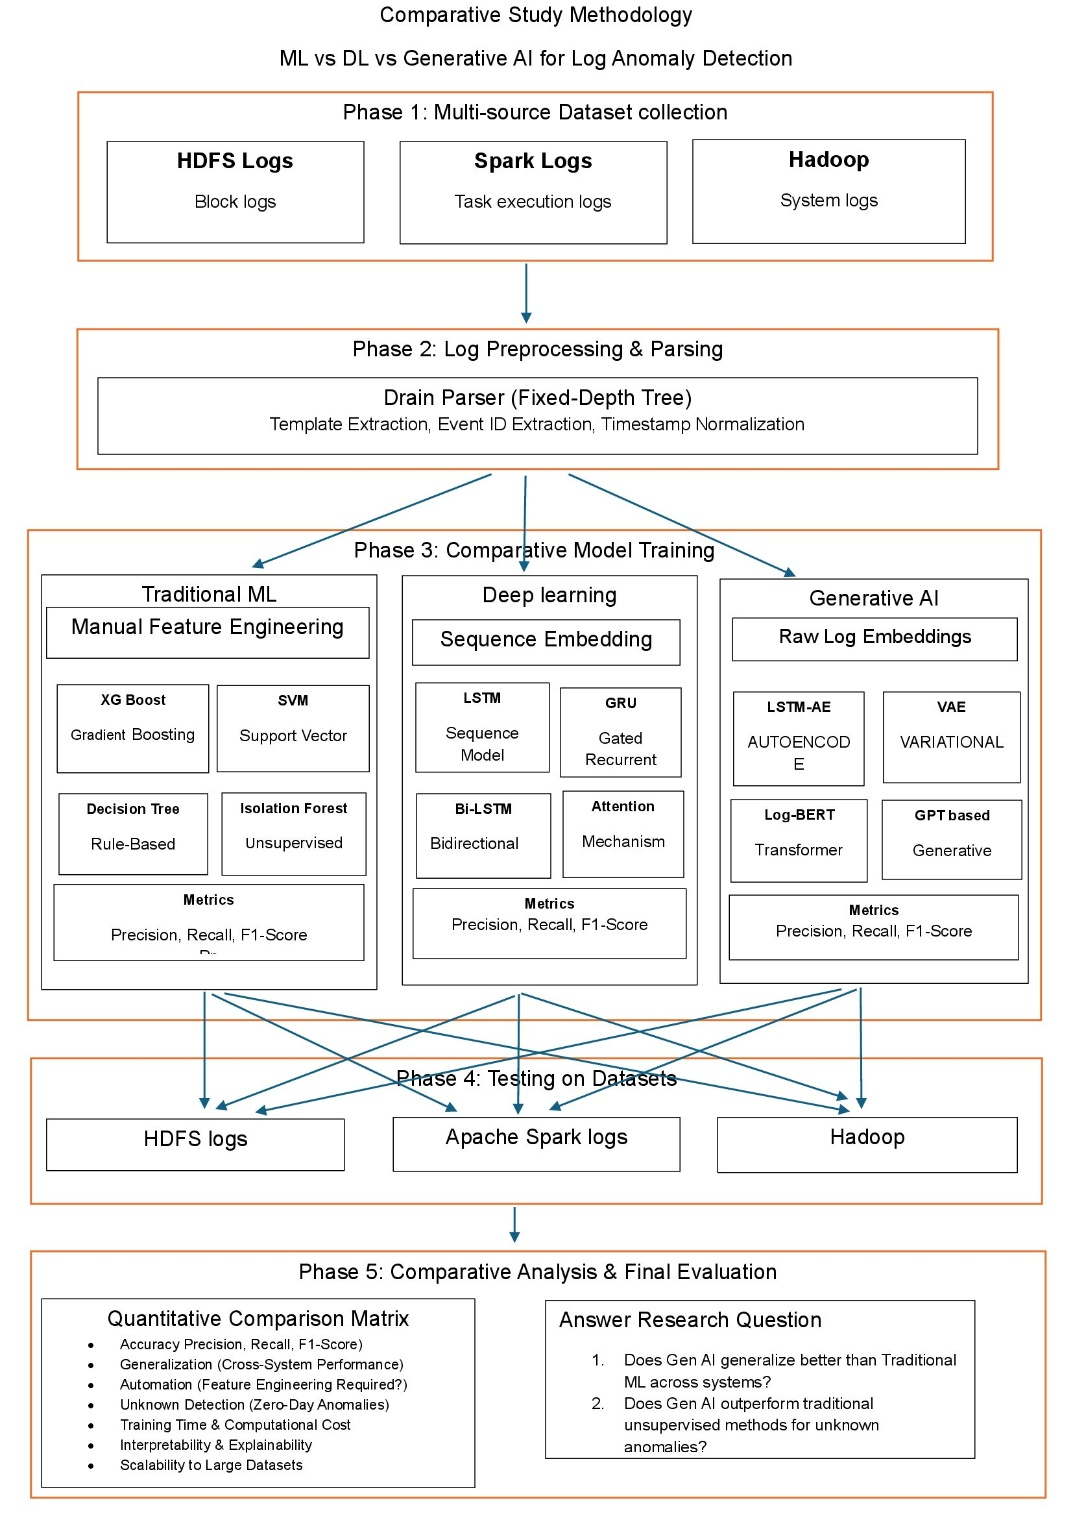
\includegraphics[width=\linewidth]{./media/2f3c9ab99b17edec963cb493396b605ade69c150.png}}
\caption{Five-phase comparative study methodology.}
\label{fig1}
\end{figure}

\subsection{Phase 1 -- Multi-Source Dataset Collection}
HDFS block logs, Apache Spark task execution logs, and Hadoop system logs form a multi-source repository for heterogeneous comparative testing.

\subsection{Phase 2 -- Log Preprocessing and Parsing}
Raw logs are processed with the Drain parser [3], a fixed-depth tree approach, performing template extraction, event ID extraction, and timestamp normalization.

\subsection{Phase 3 -- Comparative Model Architectures}
Three parallel pipelines are implemented: (i) Traditional ML (XGBoost, Random Forest, Isolation Forest) using Event Count Matrices; (ii) Deep Learning sequence models (LSTM, GRU, Bi-LSTM with attention, CNN) operating directly on log sequences; and (iii) Generative AI (VAE, GAN, LSTM-Autoencoder) trained on normal-only data using raw log embeddings, with anomaly scores derived from reconstruction probability.

\subsection{Phase 4 -- Training and Testing Dynamics}
Each model is evaluated with an 80/20 train-test split sourced from the same dataset (intra-system validation), independently repeated across HDFS, Spark, and Hadoop to verify performance consistency without cross-contaminating training distributions.

\subsection{Phase 5 -- Comparative Analysis}
Models are assessed via Precision, Recall, F1-score, ROC-AUC, and PR-AUC, alongside qualitative criteria: performance consistency, automation level, zero-day detection capability, training time, interpretability, and scalability.

\section{Results and Discussion}

\subsection{HDFS Baseline Performance}
Models were evaluated on an 80/20 split of the HDFS dataset (558,223 normal, 16,838 anomaly log vectors; 115,013-instance test set). XGBoost achieved near-perfect performance, with 5 false positives and 1 missed anomaly out of 3,368.

\begin{figure}[htbp]
\centerline{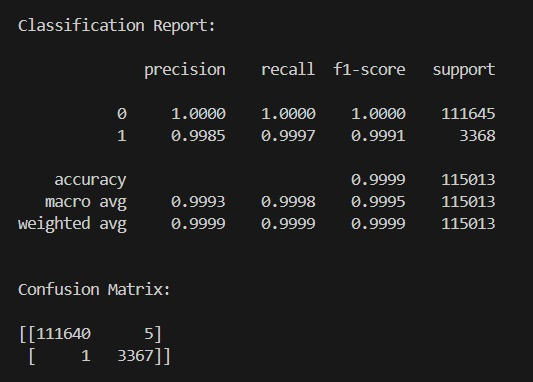
\includegraphics[width=\linewidth]{./media/2e2476b7371b6938231aa0b67cfc4504057a8dc7.png}}
\caption{HDFS ML XGBoost confusion matrix.}
\end{figure}

SVM achieved strong baseline performance (128 false positives, 2 missed anomalies), though XGBoost outperformed it across all key parameters, reflecting its superior capacity for non-linear decision boundaries.

The supervised Deep Learning pipeline evaluated sequence models without rigid manual feature engineering. LSTM produced 66 false positives and missed 4 anomalies (ROC-AUC = 1.0); GRU performed comparably, missing only 3 anomalies.

\begin{figure}[htbp]
\centerline{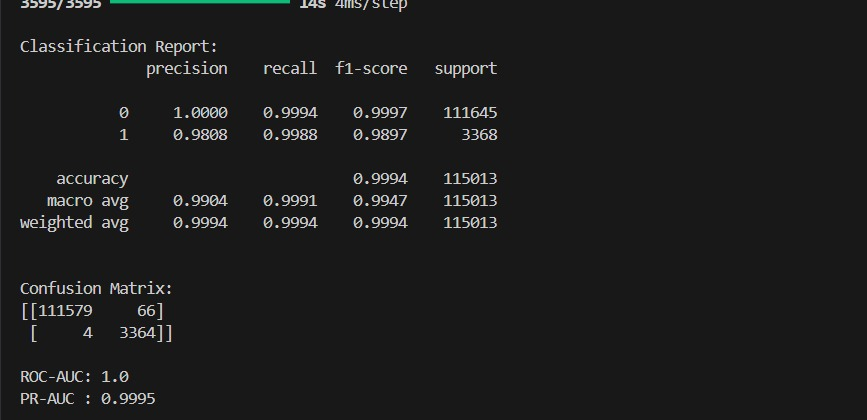
\includegraphics[width=\linewidth]{./media/baadb35db958ee3c0d4f4b3d70701c1eab3b62cd.png}}
\caption{DL LSTM confusion matrix and ROC-AUC results.}
\end{figure}

Generative AI models were trained exclusively on normal sequences. The LSTM-Autoencoder produced 1,137 false positives and 398 missed anomalies (ROC-AUC 0.9964, PR-AUC 0.9049); the LSTM-VAE produced 1,101 false positives and 866 missed anomalies (ROC-AUC 0.9876, PR-AUC 0.7854).

Table I summarizes the HDFS comparison: XGBoost and the supervised DL models (LSTM, GRU) dominate, while generative models establish a lower, but non-trivial, zero-day detection baseline.

\begin{table}[htbp]
\caption{HDFS MODEL COMPARISON}
\begin{center}
\begin{tabular}{|l|l|c|c|c|c|}
\hline
\textbf{Model} & \textbf{Type} & \textbf{Prec.} & \textbf{Recall} & \textbf{F1} & \textbf{ROC-AUC} \\ \hline
XGBoost & Trad. ML & 99.85\% & 99.97\% & 99.91\% & -- \\ \hline
SVM & Trad. ML & 96.34\% & 99.94\% & 98.11\% & -- \\ \hline
LSTM & Sup. DL & 98.08\% & 99.88\% & 98.97\% & 100.0\% \\ \hline
GRU & Sup. DL & 98.08\% & 99.91\% & 98.99\% & 100.0\% \\ \hline
LSTM-AE & Generative & 72.32\% & 88.18\% & 79.46\% & 99.64\% \\ \hline
LSTM-VAE & Generative & 69.44\% & 74.29\% & 71.78\% & 98.76\% \\ \hline
\end{tabular}
\end{center}
\end{table}

\subsection{Spark Logs Analysis}
On Apache Spark logs, Random Forest achieved the strongest ROC-AUC (0.9902), while Isolation Forest (0.9559) and One-Class SVM (0.2388) performed poorly; Isolation Forest also suffered low precision and F1 (0.04).

The LSTM-Autoencoder reached ROC-AUC 0.9822 with recall 0.93 for anomalies, but precision of only 0.02 (F1 = 0.05), reflecting severe false-positive volume.

\begin{figure}[htbp]
\centerline{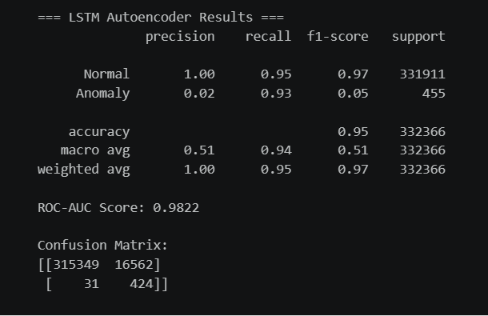
\includegraphics[width=\linewidth]{./media/35930f2015c925f2a2e3bb2d80d2b9489c19010c.png}}
\caption{LSTM results (Spark).}
\end{figure}

The CNN classifier recorded the highest overall ROC-AUC (0.9978) with perfect recall (1.00), but likewise suffered severe precision collapse (0.09), yielding F1 = 0.16.

Both generative models performed poorly on Spark: the VAE reached ROC-AUC 0.7700 with F1 = 0.01, while the GAN failed to detect anomalies effectively (ROC-AUC 0.2479, F1 = 0.01).

\subsubsection{Spark Comparative Analysis Synthesis}
The complex, overlapping nature of Spark execution logs created a massive false-positive problem: the LSTM-Autoencoder alone generated 16,562 false positives, dropping F1 to 0.05 despite a strong ROC-AUC of 0.9822. Both generative models collapsed to F1 = 0.01, indicating that Spark's structural noise and concurrency fundamentally disrupt latent-distribution mapping.

\subsection{Hadoop Logs Analysis}
On Hadoop, Random Forest achieved perfect metrics (ROC-AUC, Recall, F1 = 1.0000); this is attributable to per-application label leakage rather than genuine separability, making the Spark results more reliable for cross-dataset comparison. Isolation Forest and One-Class SVM performed poorly.

Deep learning performance was mixed on Hadoop. The CNN classifier performed strongly (ROC-AUC 0.9617, F1 = 0.91); the LSTM-Autoencoder degraded sharply relative to its Spark result (ROC-AUC 0.6519, F1 = 0.45).

Generative models remained weak on Hadoop: the GAN achieved ROC-AUC 0.6133 (F1 = 0.03), while the VAE recorded ROC-AUC 0.5235 (F1 = 0.12).

\begin{figure}[htbp]
\centerline{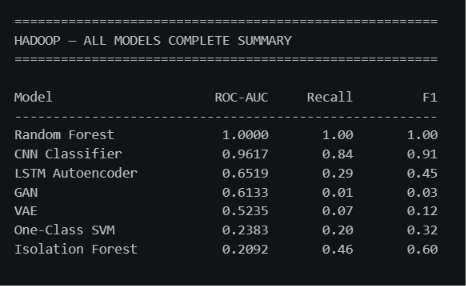
\includegraphics[width=\linewidth]{./media/9bbb6db67ea29b103fefb702d09dfb52fc9be0c5.png}}
\caption{Hadoop --- all-model results summary.}
\end{figure}

\subsection{Overall Performance Synthesis}
Table II summarizes F1-scores across all three datasets. Random Forest is the most consistently reliable model overall; CNN shows excellent ROC-AUC but highly dataset-dependent F1 (0.16 on Spark vs. 0.91 on Hadoop); Generative and unsupervised models remain consistently weak across environments.

\begin{table}[htbp]
\caption{OVERALL MODEL F1-SCORES ACROSS DATASETS}
\begin{center}
\begin{tabular}{|l|l|c|c|c|}
\hline
\textbf{Model} & \textbf{Category} & \textbf{HDFS} & \textbf{Spark} & \textbf{Hadoop} \\ \hline
XGBoost & Trad. ML (S) & 0.9991 & -- & -- \\ \hline
SVM & Trad. ML (S) & 0.9811 & -- & -- \\ \hline
Random Forest & Trad. ML (S) & -- & 0.44 & 1.00 \\ \hline
LSTM & DL (Sup.) & 0.9897 & -- & -- \\ \hline
GRU & DL (Sup.) & 0.9899 & -- & -- \\ \hline
CNN & DL (Sup.) & -- & 0.16 & 0.91 \\ \hline
Isolation Forest & Trad. ML (U) & -- & 0.04 & 0.60 \\ \hline
One-Class SVM & Trad. ML (U) & -- & 0.00 & 0.32 \\ \hline
LSTM-AE & Generative & 0.7946 & 0.05 & 0.45 \\ \hline
VAE & Generative & 0.7178 & 0.01 & 0.12 \\ \hline
GAN & Generative & -- & 0.01 & 0.03 \\ \hline
\end{tabular}
\end{center}
\end{table}

Three key patterns emerge. First, the "HDFS illusion": nearly every model performs exceptionally well on HDFS, suggesting the anomaly-detection problem is largely solved---an impression that does not generalize. Second, the Spark reality check: the complex, overlapping nature of Spark execution logs collapses F1-scores below 0.50 for almost every model despite strong ROC-AUC values. Third, the generative struggle: while theoretically advantageous for removing manual feature engineering, Generative AI consistently underperforms across all environments, peaking at F1 = 0.7946 on HDFS and failing on Spark and Hadoop.

\section{Conclusion and Future Work}
This paper presented a comparative study of Traditional ML, Deep Learning, and Generative AI for automated log anomaly detection across HDFS, Apache Spark, and Hadoop. The findings reveal a clear trade-off between accuracy and functional autonomy: traditional supervised classifiers achieve near-perfect F1-scores on structurally consistent datasets but depend on manual feature engineering; supervised deep sequence models remove this dependency while matching accuracy, yet degrade under Spark's noise and concurrency; and Generative AI, despite consistently high ROC-AUC, achieves lower F1-scores overall, establishing only a baseline capability for zero-day anomaly discovery rather than outright superiority over supervised approaches.

Future work will explore dynamic thresholding (e.g., extreme value theory) to reduce false positives in generative models, online incremental learning for concept-drift mitigation, fine-grained parsing of variable log fields, and hybrid neuro-symbolic frameworks combining ensemble robustness with generative flexibility.

\section*{Acknowledgment}
The author thanks Prof. Dr. Imran Ihsan for his supervision and guidance throughout this research.

\begin{thebibliography}{00}
\bibitem{b1} J. Zhu, S. He, P. He, J. Liu, and M. R. Lyu, ``Loghub: A large collection of system log datasets for AI-driven log analytics,'' in \textit{Proc. IEEE 34th Int. Symp. Software Reliability Engineering (ISSRE)}, 2023, pp. 355--366.
\bibitem{b2} W. Meng et al., ``LogAnomaly: Unsupervised detection of sequential and quantitative anomalies in unstructured logs,'' in \textit{Proc. 28th Int. Joint Conf. Artificial Intelligence (IJCAI)}, 2019, pp. 4739--4745.
\bibitem{b3} P. He, J. Zhu, Z. Zheng, and M. R. Lyu, ``Drain: An online log parsing approach with fixed depth tree,'' in \textit{Proc. IEEE Int. Conf. Web Services (ICWS)}, 2017, pp. 33--40.
\bibitem{b4} M. Du, F. Li, G. Zheng, and V. Srikumar, ``DeepLog: Anomaly detection and diagnosis from system logs through deep learning,'' in \textit{Proc. ACM SIGSAC Conf. Computer and Communications Security}, 2017, pp. 1285--1298.
\bibitem{b5} X. Zhang et al., ``Onion: Identifying incident-indicating logs for cloud systems,'' in \textit{Proc. 29th ACM Joint Meeting European Software Engineering Conf. and Symp. Foundations of Software Engineering (ESEC/FSE)}, 2021, pp. 1253--1263.
\bibitem{b6} W. Xu, L. Huang, A. Fox, D. A. Patterson, and M. I. Jordan, ``Detecting large-scale system problems by mining console logs,'' in \textit{Proc. ACM SIGOPS 22nd Symp. Operating Systems Principles (SOSP)}, 2009, pp. 117--132.
\bibitem{b7} F. T. Liu, K. M. Ting, and Z. H. Zhou, ``Isolation forest,'' in \textit{Proc. 8th IEEE Int. Conf. Data Mining (ICDM)}, 2008, pp. 413--422.
\bibitem{b8} Q. Lin, H. Zhang, J. G. Lou, Y. Zhang, and X. Chen, ``Log clustering based problem identification for online service systems,'' in \textit{Proc. 38th Int. Conf. Software Engineering Companion (ICSE-C)}, 2016, pp. 102--111.
\end{thebibliography}

\end{document}